\documentclass[11pt]{beamer}
\title{Array Fold Logic}
\usepackage{verbatim}
\usepackage{amsmath}
\usepackage{amsthm}
\usepackage{listings}
\usepackage{graphics}
\usepackage{color}
\usepackage{stmaryrd}\usefonttheme[onlymath]{serif}

\newtheorem{proposition}{Proposition}
\author{Przemyslaw Daca et al.}
\date{\today}


\begin{document}
\maketitle
\begin{frame}\frametitle{Overview }
\begin{itemize}

\item Contributions of this paper.
\item Array fold logic: syntax, semantics and utilities.
\item Theoretical results.
\item Tool and experimental results.

\end{itemize}
\end{frame}


\begin{frame}\frametitle{Array Fold Logic: Syntax}
\textbf{Implicit Variables:} $\{\textbf{e}, \textbf{c}_1, \ldots, \textbf{c}_{m-1}, \textbf{i}\} = FV^{m}$

\begin{itemize}
\item Array sort, \texttt{ASort}
\item Integer sort, \texttt{ISort}
\item Boolean sort, \texttt{BSort}
\item Integer vectors $\texttt{VSort}^m$
\item Functional constants $\texttt{FSort}^m = \texttt{VSort}^m\times \texttt{ISort}\rightarrow \texttt{VSort}^m$
\end{itemize}
\end{frame}

\begin{frame}\frametitle{Array Fold Logic: Syntax}

\begin{center}
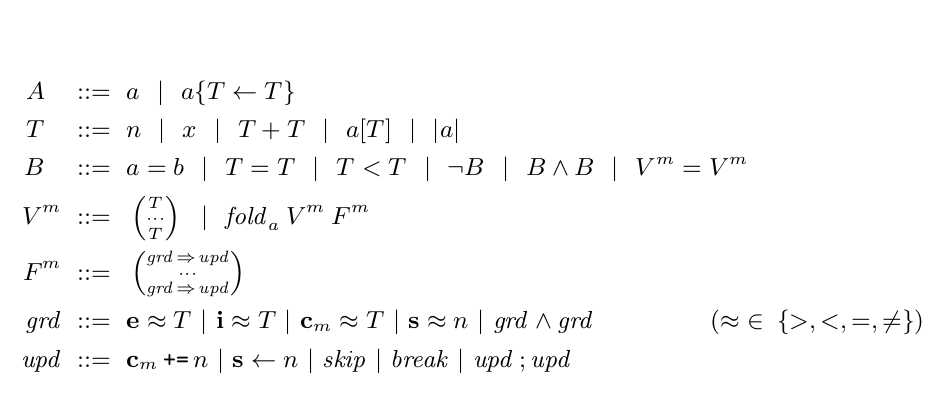
\includegraphics[scale=0.32]{aflsyn.png}
\end{center}

Given a set of function branches $Br$, we can define a control flow graph $G =\langle S,E,\gamma \rangle $.
\begin{itemize}
\item $E = \bigcup_{grd\Rightarrow upd \in Br} \{(s_1, s_2)\mid s_1 \models grd\wedge s_2 = ite(\textbf{s}\leftarrow n\in upd, n, s_1)\}$
\item $\gamma$ is the labeling of edges with the set of formulas $\Phi(grd)$ and $\Phi(upd)$.
\end{itemize}
Requirement: edges in the same SCC of $G$ update the counters in a monotonic way.

\end{frame}

\begin{frame}\frametitle{Array Fold Logic: Semantics}
$\sigma = \langle\lambda, \mu\rangle$ where $\mu: Var_{I} \rightarrow \mathbb{Z}, \lambda: Var_{A} \rightarrow \mathbb{Z}^*$.

$\kappa = FV^{m} \rightarrow \mathbb{Z}^{m+1}$
\begin{center}
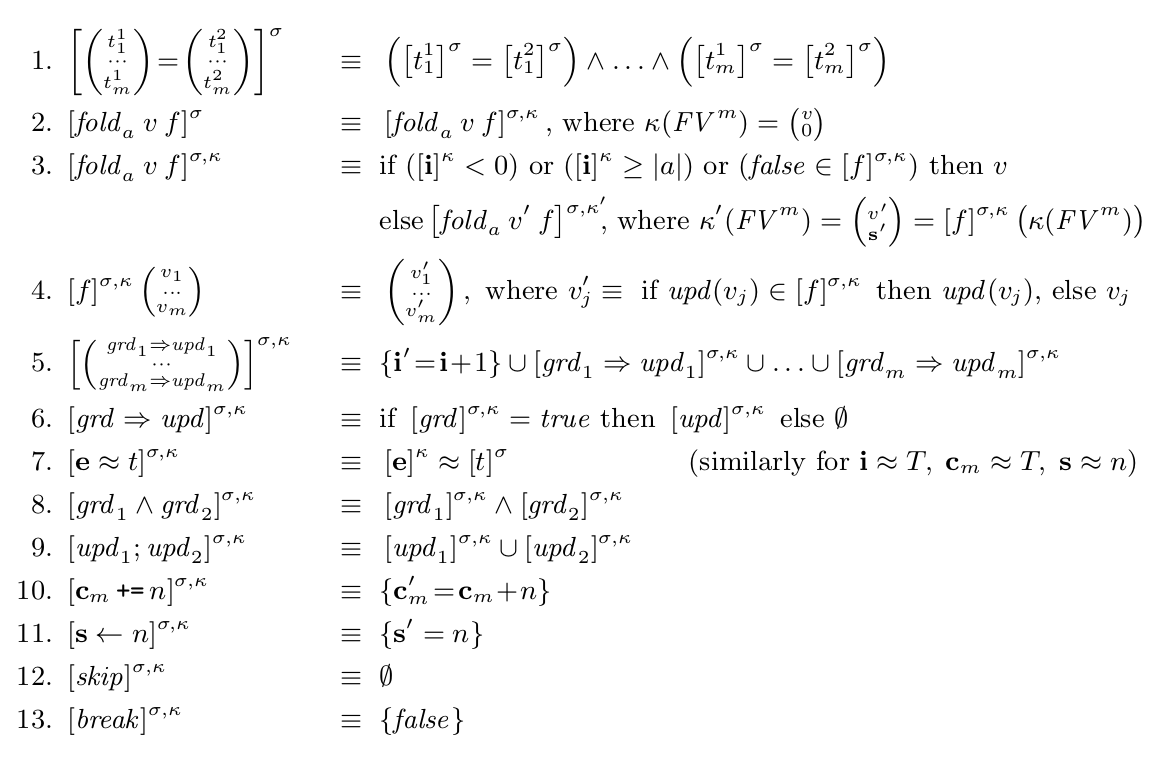
\includegraphics[scale=0.26]{aflsema.png}
\end{center}

\end{frame}

\iffalse
\begin{frame}\frametitle{Utility and Expressive Power}
\begin{itemize}
\item Boundedness:
\[fold_a(0)(l\le \textbf{e} \le u \Rightarrow skip) = |a|\]
\item Partitioning:
\begin{center}
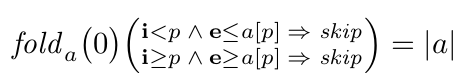
\includegraphics[scale=0.36]{partitionafl.png}
\end{center}
\item Periodic:
\begin{center}
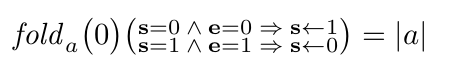
\includegraphics[scale=0.36]{periodicafl.png}
\end{center}
\item Pumping($0^n1^n$):
\begin{center}
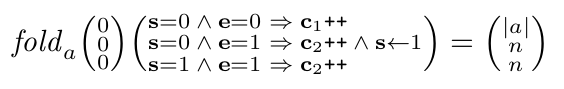
\includegraphics[scale=0.36]{pumpingafl.png}
\end{center}
\item Counting.
\item Histogram.
\end{itemize}
Properties that require universal quantification over \textit{several} index variables are inexpressive.
e.g. Sortedness and ...
 \end{frame}
 
 \fi
\begin{frame}\frametitle{Theoretical Results: Complexity}
\begin{definition}[symbolic $k$-counter machine]

An SMC is a tuple $\mathcal{M} = (\vec{\eta}, X, Q, \delta, q^{init})$ where 
\begin{itemize}
\item $\vec{\eta}$ is a vector of k counters $\eta_1, \ldots,\eta_n$.
\item $X$ is a finite set of integer variables.
\item $Q$ is a finite set of states.

\item $\delta \subseteq Q\times \texttt{CC}_k(X) \times \texttt{IC}(X)\times Q\times \mathbb{Z}^k$ is the transition relation.

\item $q^{init} \in Q$ is the initial state.

\end{itemize}
\end{definition}
The effect of a transition $(q_1, \alpha, \beta, q_2, \kappa)\in \delta$. 

Input constraints $\texttt{IC}(X)$.

Counter constraints $\texttt{CC}_k(X)$, here $k$ means the counters are no greater than $k$.

\end{frame}

\begin{frame}\frametitle{Reversal and Reversal-Bounded}
\begin{definition}[Reversal]
A counter machine makes a \textit{reversal} if it makes an alternation between non-increasing and non-decreasing some counter.

A machine is \textit{reversal-bounded} if there exists a constant $c\ge 0$ such that on all accepting runs every counter makes at most $c$ reversal.
\end{definition}

\begin{example}
Assume there is only one counter.

$\textbf{1,2,3,3,4},3,2,2,\textbf{3,5},3,1$



\end{example}
\end{frame}

\begin{frame}\frametitle{Translation from Function to SCM}

Translation from a functional constant $f$ of $\texttt{FSort}^m$ to an SCM.

\begin{definition}
We define the translation of functional constant $f$ of sort $\texttt{FSort}^m$ ocurring in a formula $\phi$, as an SCM $\mathcal{M}(f) = (\vec{\eta}, X, Q, \delta, q^{init})$. Let $G = \langle G,E,\gamma\rangle$ be the CFG defined before, then $\vec{\eta} = \{\mathbf{i, c_1, \ldots, c_m}\}$, $X$ are fresh free variables for each integer term $T$ in $f$, $Q = S$, $q^{init} = 0$. For transitions the formula are translated from $\Phi(grd)$ and $\Phi(upd)$ in $G$.

\end{definition}


The translated SVM is reversal bounded. Why?

\[SCC_1 \rightarrow SCC_2 \rightarrow\cdots \rightarrow SCC_m\]

\end{frame}

\begin{frame}\frametitle{
Parallel composition of SCMs}
\begin{center}
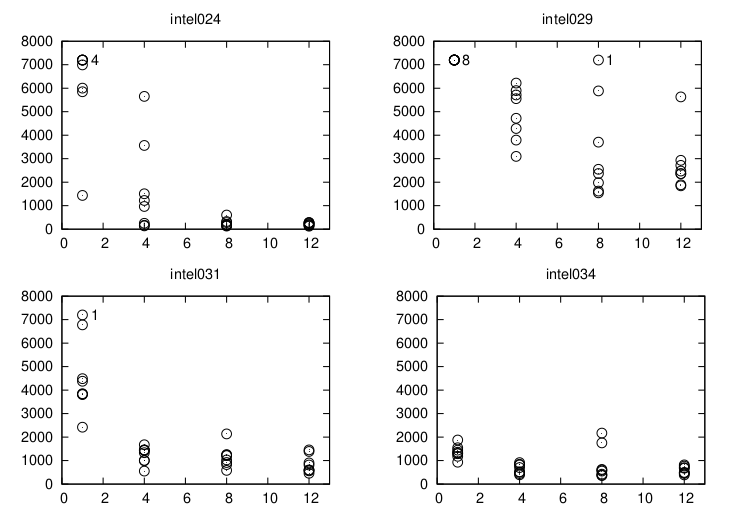
\includegraphics[scale=0.28]{para.png}
\end{center}

\end{frame}

\begin{frame}\frametitle{Small model property}
\begin{lemma}
There exists a constant $c\in \mathbb{N}$, such that an AFL formula $\Phi$ is satisfiable iff there exists a model $\sigma$ it maps each variable in $X$ to integer that $\le 2^{|\Phi|^c}$ and array to sequence of $\le 2^{|\phi|^c}$ where each integer of the array also lies in the bound.
\end{lemma}

Give fixed counter values.

Why we want reversal-bounded?

\begin{theorem}
The satisfiability problem of AFL is \textbf{PSPACE}-complete.

\end{theorem}
Membership: NTM.

Hardness: DFA emptiness problem reduced to sat of AFL formula.

\end{frame}

\begin{frame}\frametitle{Undecidable Extension}
\begin{theorem}
Array fold logic with $\exists^*\forall^*$ extension is undecidable. 
\end{theorem}

\begin{proof}
Reduction from Hilbert's Tenth Problem to the decidability of quantified AFL. $x = y\cdot z$.
\begin{center}

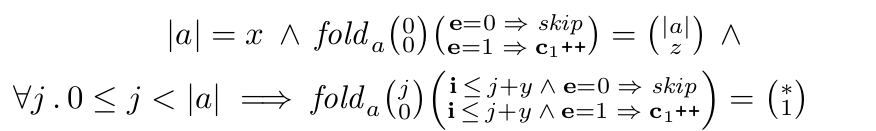
\includegraphics[scale=0.34]{undeafl.png}

\end{center}
\end{proof}
\end{frame}

\begin{frame}\frametitle{Decision Procedure}
Idea: translate the AFL formula $\phi$ into a quantifier-free PA formula $\psi = \psi_n \wedge \psi_e \wedge \psi_l$.

\begin{itemize}
\item $\psi_n$ is part of $\phi$ that does not contain fold.
\item $\psi_e$ is the reduction from the reachability problem of SMC to QFPA.
\item $\psi_l$ is the link formula used for linking some constraints between initial and final configuration in $\psi_e$.
\end{itemize}

\begin{lemma}
The complexity of satifiability of $m$-AFL for a fixed $m$ is \textbf{NP}-complete.
\end{lemma}

\end{frame}

\end{document}